\documentclass[a4paper,12pt]{article}

\usepackage[top=3cm, bottom=2cm, left=3cm, right=2cm]{geometry}
\usepackage[utf8]{inputenc}
\usepackage[portuguese]{babel}
\usepackage{booktabs}
\usepackage{multirow}
\usepackage{hyperref}
\usepackage{graphicx}
\usepackage{longtable}
\usepackage{verbatim}

\usepackage{float}
\floatstyle{ruled}
\newfloat{program}{thp}{lop}
\floatname{program}{Script}

\title{Serviços de Rede e de Sistema \\
Interior Routing }

\author{André Fernandes (ei03107) \and Miguel Gomes (ei07075) \and Pedro Batista (ext10392)}

\begin{document}

\maketitle

\section{Topologia}
A topologia de rede implementada foi exatamente igual a proposta do relatório. Esta é mostrada na Figura~\ref{fig:topologia}.

\begin{figure}[htp]
	\begin{center}
		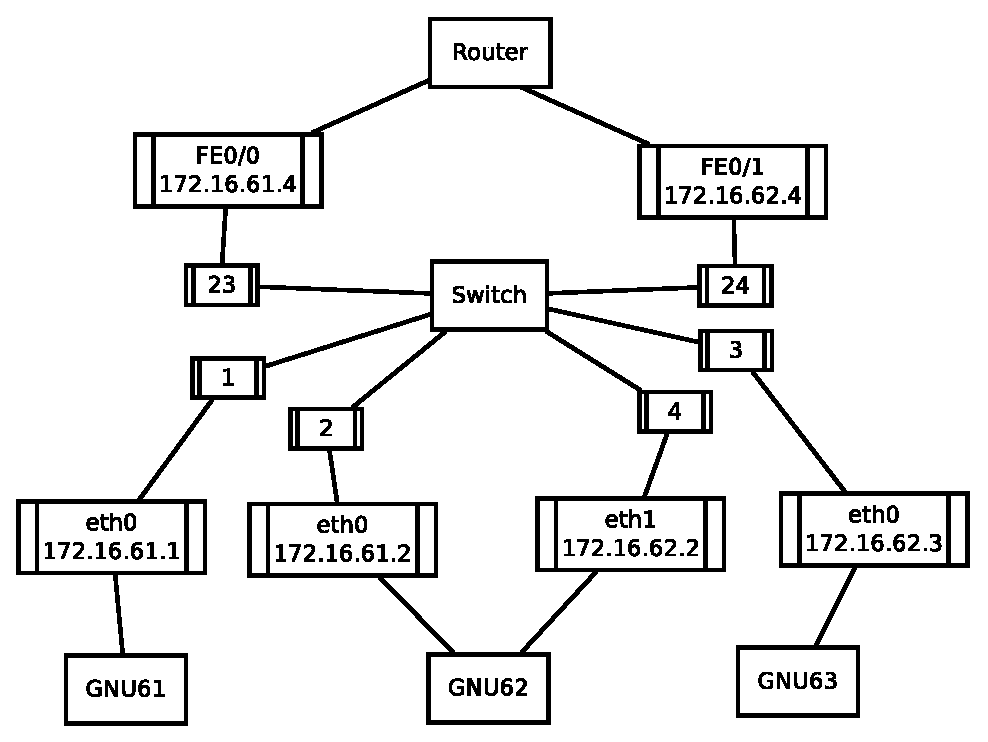
\includegraphics[height=4in]{topologia}
	\end{center}
	\caption{Topologia de rede impelementada.}
	\label{fig:topologia}
\end{figure}

\section{Cenários}

\section{Análise de Tráfego}

	Com o objectivo de capturar o tráfego completo da rede configurámos as capacidades Switched Port Analyzer (SPAN) do switch. Esta configuração permitiu que uma porta do switch servisse para receber dados de monitorização de todo o tráfego da rede, independentemente da VLAN em que os pacotes surjam.


%PSB: comentei pra poder compilar
%	\begin{figure}[htp]
%   	\begin{center}
%	 		\includegraphics[height=300pt]{}
%		\end{center}
%		\caption{}
%		\label{fig:}
%	\end{figure}

\section{Arquivos de log}
Na pasta logs anexada a este arquivo, podemos encontrar os logs e arquivos de
configuração capturados. Para este assumimos a seguinte convenção \verb gX  para
os Gnus (\verb X  representa o respectivo Gnu), \verb r6  para o router cisco, e
\verb s6  para o switch cisco. As pastas \verb logs/cY  representas os três
cenários indicados no guia (\verb Y  varia de 1 a 3 representando os cenários).
Já as pastas \verb logs/cY/trace_route  como o nome indica representa o
trace route de todos os componentes para todos os outros do sistema. Finalmente
as pastas \verb logs/conf/{gX,r6,s6}  mostram as configurações efetuadas no
sistema. Abaixo detalhamos os arquivos de cada pasta.

\begin{itemize}
	\item Para os logs em \verb-logs/cY-
		\begin{description}
			\item \verb *\_zebra  Representa o comando \verb-show ip route-.
			\item \verb *\_ospf  Representa o comando \verb-show ip ospf neighbor-.
		\end{description}
	\item Para os trace routes em \verb-logs/cY/trace_route-
		\begin{description}
			\item \verb {gX,r6}_{gX,r6}[.{61,62}]  Representa o trace route do
				elemento anterior ao \verb _  para o elemento posterior. A parte
				opicional que contém o \verb .  ilustra para o caso do \verb g2  e
				\verb r6  ondo o trace route pode ser feito a rede \verb 61  ou \verb 62 .
		\end{description}
	\item Para as configurações em \verb-logs/confs/gX-
		\begin{description}
			\item[zebra.conf] Apresenta a configuração do zebra no respectivo
				gnu.
			\item[ospfd.conf] Apresenta a configuração ospf no respectivo gnu.
		\end{description}
	\item Para as configurações em \verb-logs/confs/{r6,s6}-
		\begin{description}
			\item[running-config] Apresenta a configuração do router ou switch
				gerada com o comando \verb_show running-config_.
		\end{description}
\end{itemize}


\section{Referências}

SPAN: \url{http://www.cisco.com/en/US/products/hw/switches/ps708/products_tech_note09186a008015c612.shtml#terms}

\end{document}
